\chapter{Результаты}
\label{chapter_results}

В данной главе приводятся результаты тестирования разработанных методов на модельных задачах. В качестве модельных использовались известные задачи числовой оптимизации, решаемые с помощью $(\mu + \lambda)$-эволюционной стратегии. Приводятся результаты сравнения существующих методов с существующими методами настройки параметров ЭА с помощью обучения с подкреплением. Также исследуется эффективность существующих методов выделения состояний среды.

В качестве особи рассматривался набор вещественных чисел, соответствующий размерности решаемой задачи. Для $(\mu + \lambda)$-эволюционной стратегии необходимо определить только оператор мутации. В процессе тестирования применялся следующий оператор:
\begin{equation}
 \begin{pmatrix} x_1 \\ .. \\ x_n \end{pmatrix} = \begin{pmatrix} x_1 \\ .. \\ x_n \end{pmatrix} + \sigma \begin{pmatrix}dx_1 \\ .. \\ dx_n\end{pmatrix}, dx_i \sim \mathcal{N}(0, 1)
\end{equation}

Соответственно $\sigma$ -- \textit{шаг} мутации -- является настраиваемым параметром. Значения параметра неотрицательны и задаются некоторым диапазоном вида $[0, k]$. Размер диапазона варьировался в рамках проводимого исследования. Ожидаемым поведением является уменьшение шага мутации при приближении к оптимуму.

\section{Сфера}

Необходимо с точностью $\epsilon$ найти минимум унимодальной сферической функции~(\ref{sphere_eq}).
\begin{equation}
\label{sphere_eq}
f(x_1,..,x_n) = \sum\limits_{i=1}^n{x_i^2}
\end{equation}
График функции для двух переменных представлен на рис.~\ref{sphere_plot}. При $x_i \in [-80; 120]$ глобальный минимум достигается в точке $(0,..,0)$.

\begin{figure}
    \centering
    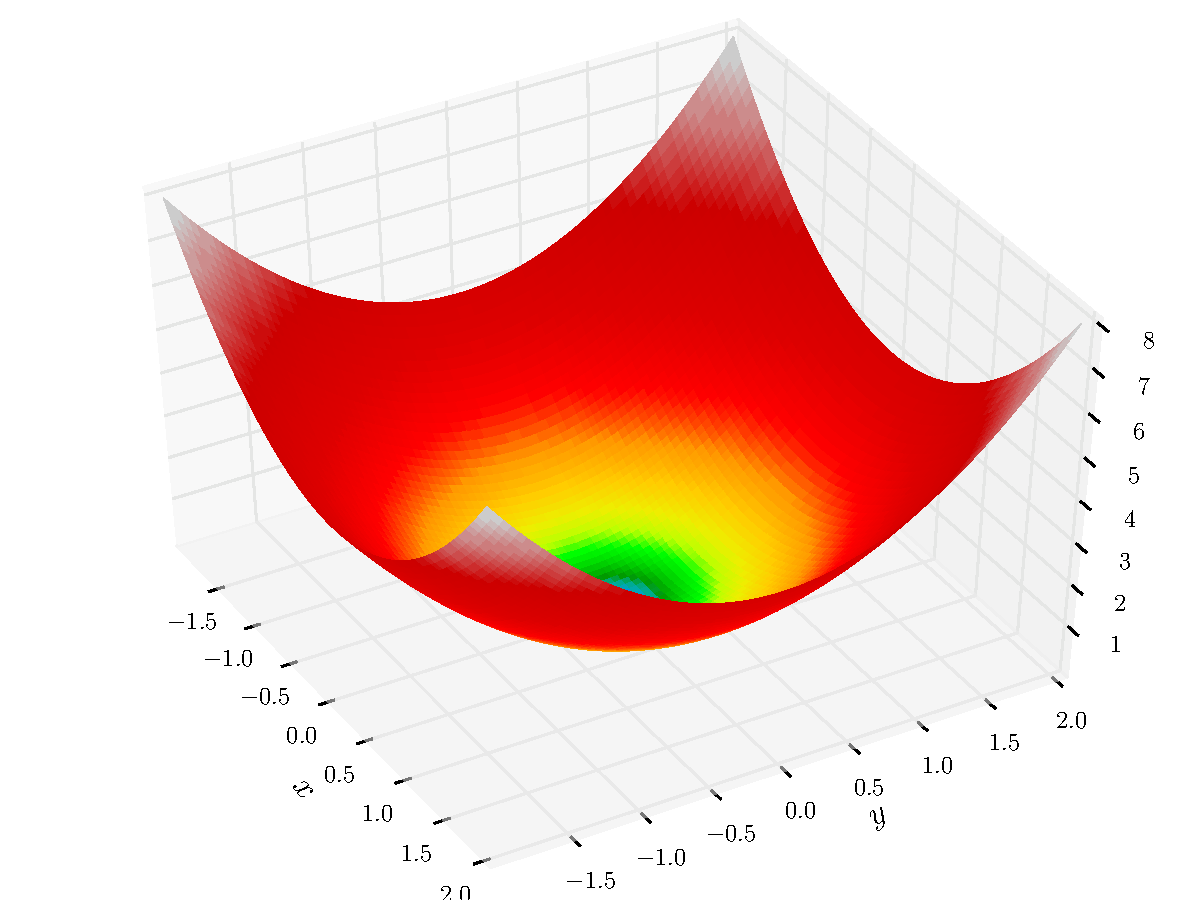
\includegraphics[width=0.6\textwidth]{sphere.pdf}
    \caption{График сферической функции для двух переменных.}
    \label{sphere_plot}
\end{figure}

\begin{figure}
    \centering
    \label{earpc_sphere_dist}
    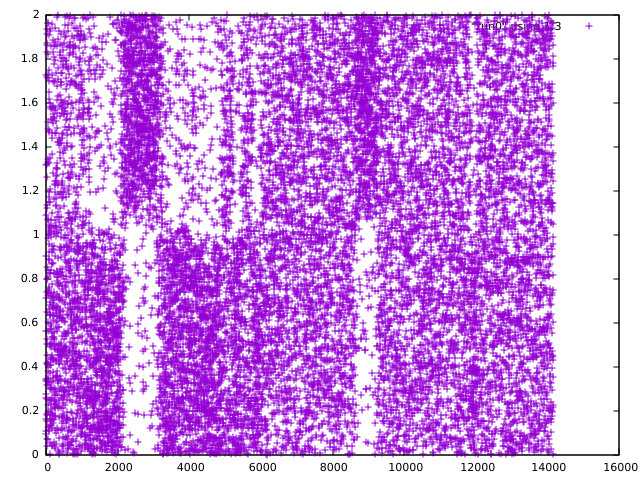
\includegraphics[width=0.6\textwidth]{earpc_sphere_dist.png}
    \caption{График выбранных значений $\sigma$ с помощью метода \textit{earpc}}
\end{figure}


\begin{figure}
\label{earpc_sphere}
    \centering
    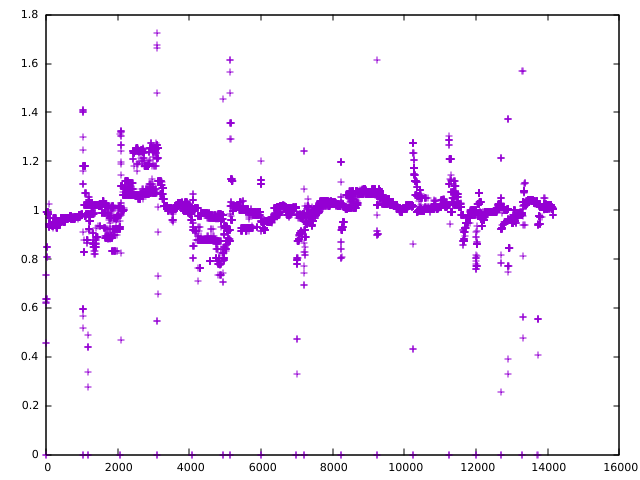
\includegraphics[width=0.6\textwidth]{earpc_sphere.png}
    \caption{График точки разбиения в методе \textit{earpc}}
\end{figure}

\begin{figure}
\label{dist_sphere}
    \centering
    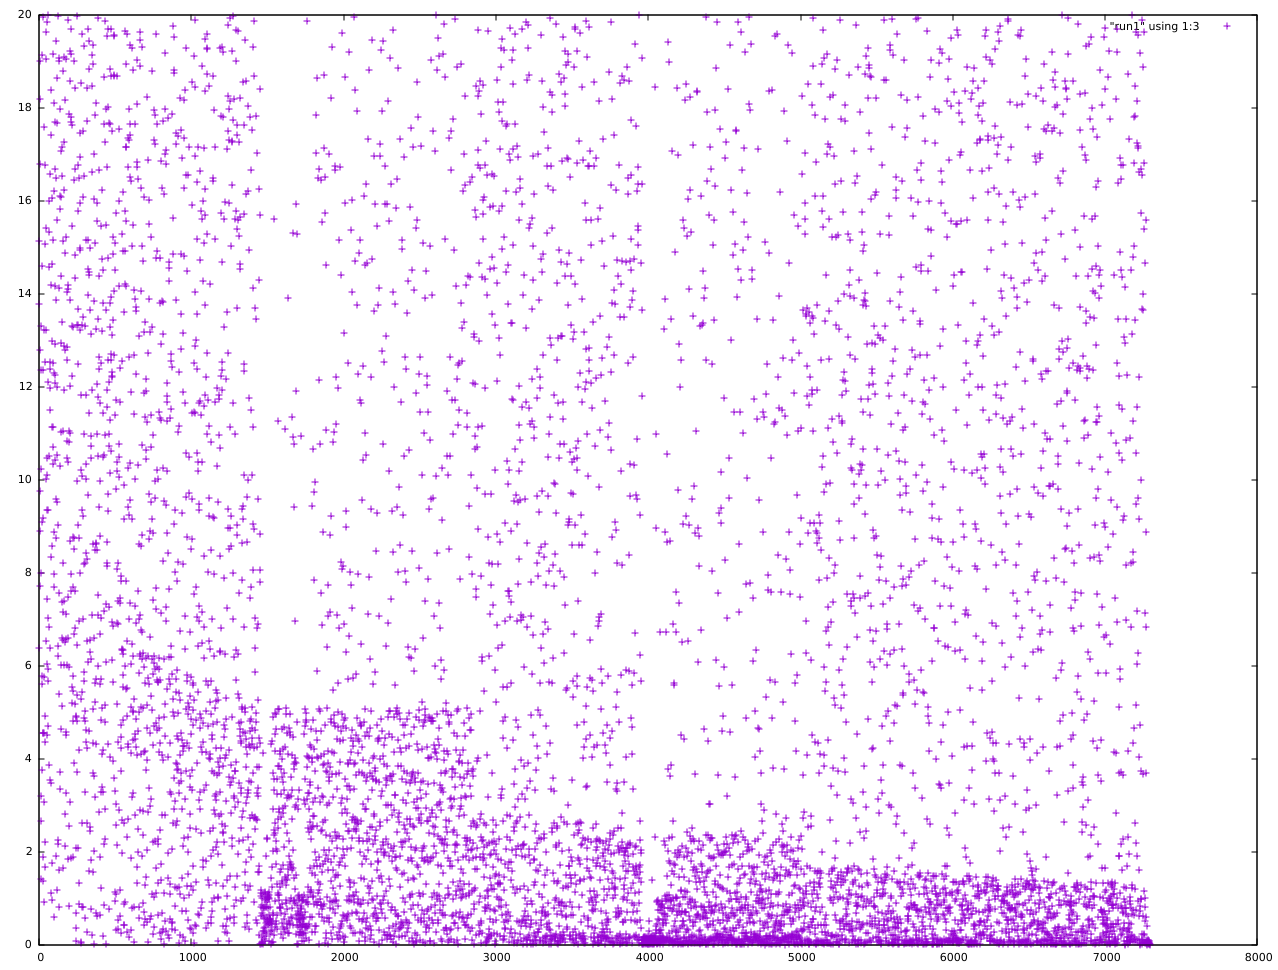
\includegraphics[width=0.6\textwidth]{dist_sphere_dist.png}
    \caption{График выбранных значений $\sigma$ с помощью предложенного метода}
\end{figure}

\begin{figure}
    \centering
    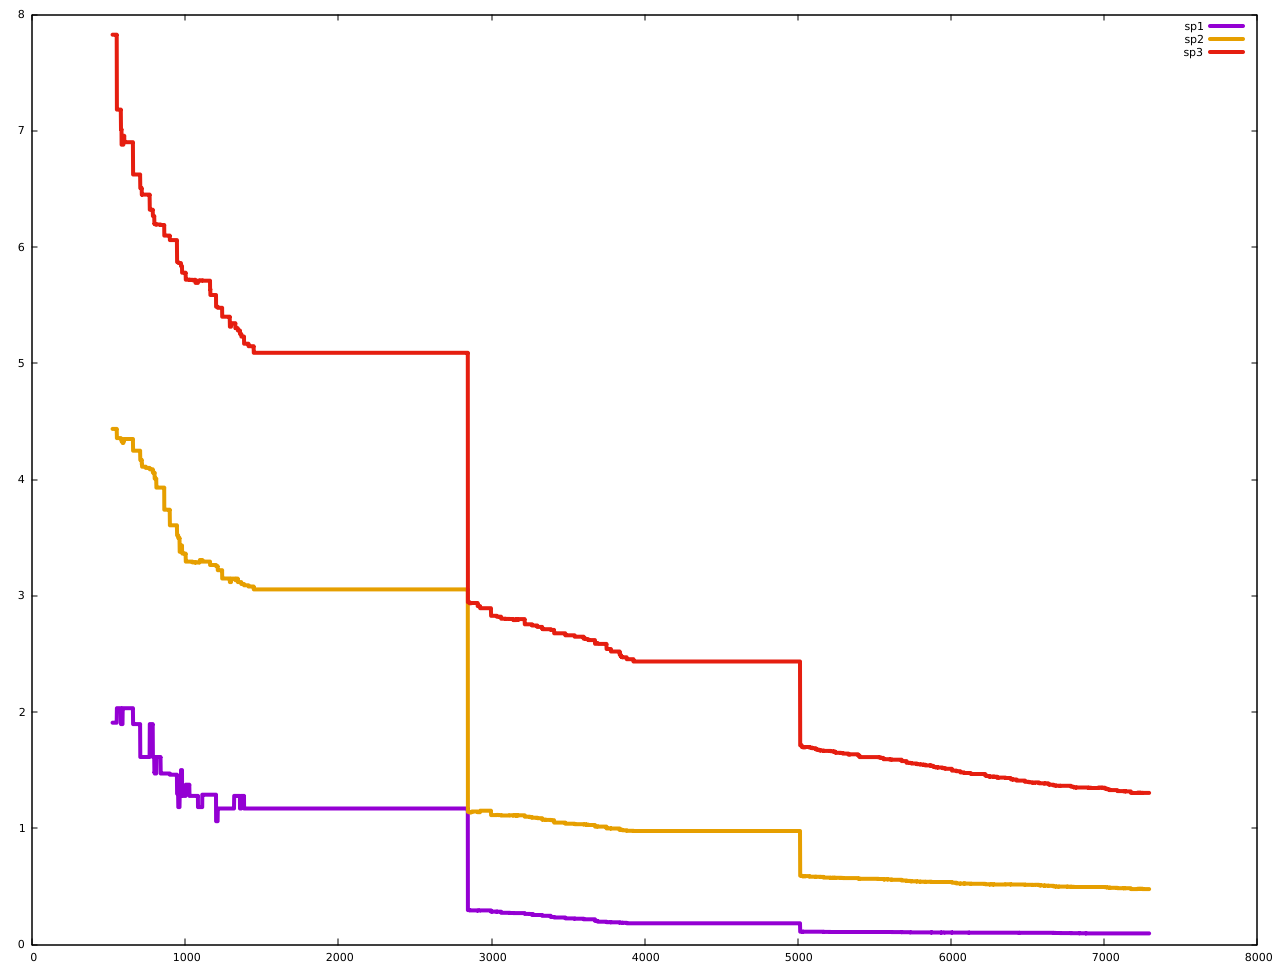
\includegraphics[width=0.6\textwidth]{dist_sphere.png}
    \caption{График точек разбиения в предложенном методе}
\end{figure}


\begin{table}
\label{sphere_results}
  \centering
  \begin{tabular}{|l|l|l|l|l|l|}
    \hline
    k & Dist & q & single q & earpc & single earpc\\
    \hline
    1 & 5372 & 13604 & 9907 & 13868 & 10996 \\
    \hline
    5 & 10058 & 54608 & 43692 & 41712 & 47427 \\
    \hline
    10 & 11964 & 67218 & 174344 & 114524 & 89886 \\
    \hline
    20 & 8876 & 178021 & 121354 & 159028 & - \\
    \hline
  \end{tabular}
  \captionsetup{justification=centering}
    \caption{Таблица с результатами}
\end{table}


\section{Функция Розенброка}


Предложенная Ховардом Розенброком невыпуклая функция~(\ref{rosenbrock_eq}) часто используется для оценки производительности алгоритмов оптимизации. Обычно $a = 1$, $b = 100$. Считается, что поиск глобального минимума для данной функции является нетривиальной задачей. График функции для двух переменных представлен на рис.~\ref{rosenbrock_plot}. Глобальный минимум находится в длинной, узкой \textit{впадине}, найти которую обычно не составляет труда. Трудность заключается в поиске минимума в этой впадине. При $x_i \in [-120; 80]$ он достигается в точке $(1,..,1)$.

\begin{equation}
\label{rosenbrock_eq}
f(x_1, x_2) = (a - x_1^2)^2 + b(x_2 - x_1^2)^2
\end{equation}


\begin{figure}
    \centering
    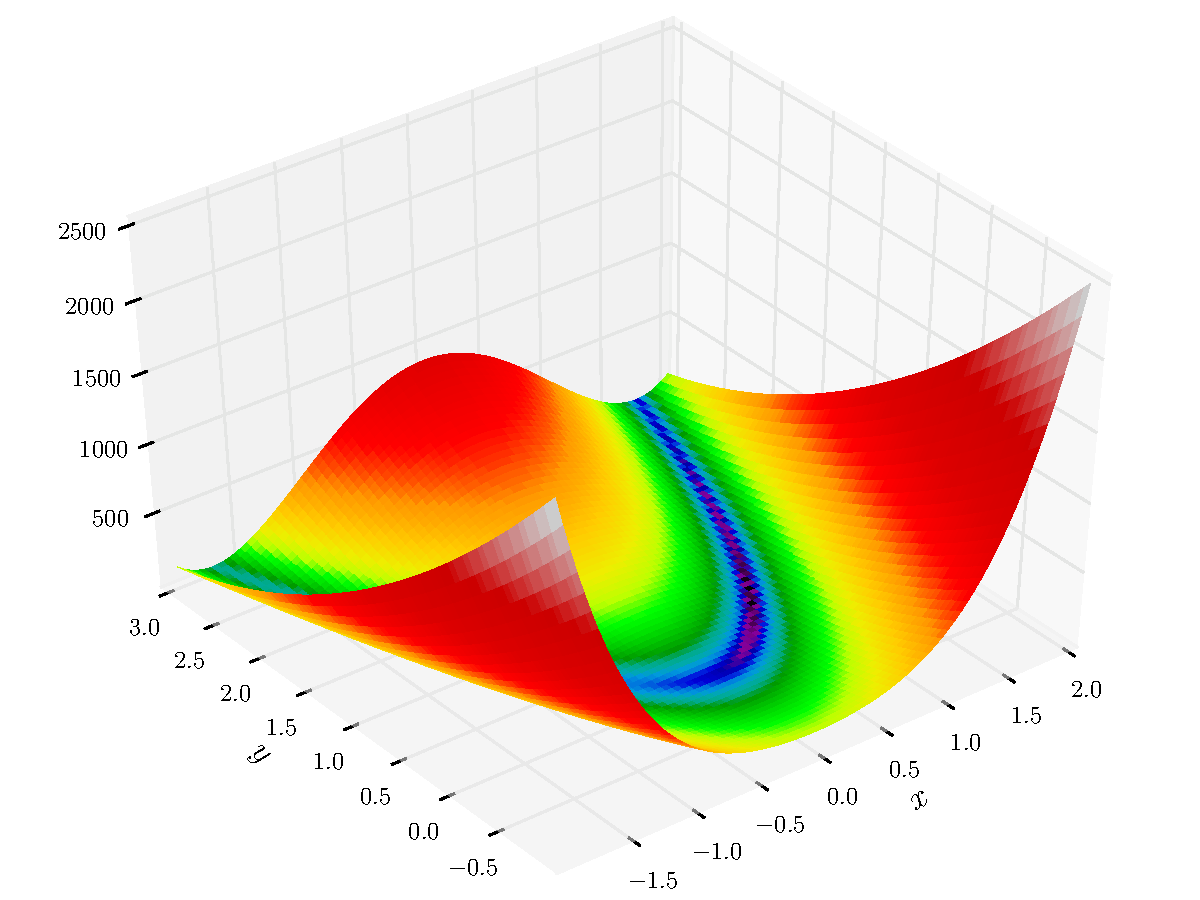
\includegraphics[width=0.6\textwidth]{rosenbrock.pdf}
    \caption{График функции Розенброка для двух переменных.}
    \label{rosenbrock_plot}
\end{figure}

\section{Функция Леви}

Мультимодальная функция Леви для двух переменных задается формулой~(\ref{levi_eq}). График функции представлен на рис.~\ref{levi_plot}. При $x, y \in [-10; 10]$ минимум достигается в точке $(1, 1)$.

\begin{equation}
\label{levi_eq}
\begin{split}
f(x_1, x2) = &sin^2(3\pi x) + (x - 1)^2(1 + sin^2(3\pi y)) + \\
& + (y - 1)^2(1 + sin^2(2\pi y))
\end{split}
\end{equation}

\begin{figure}
    \centering
    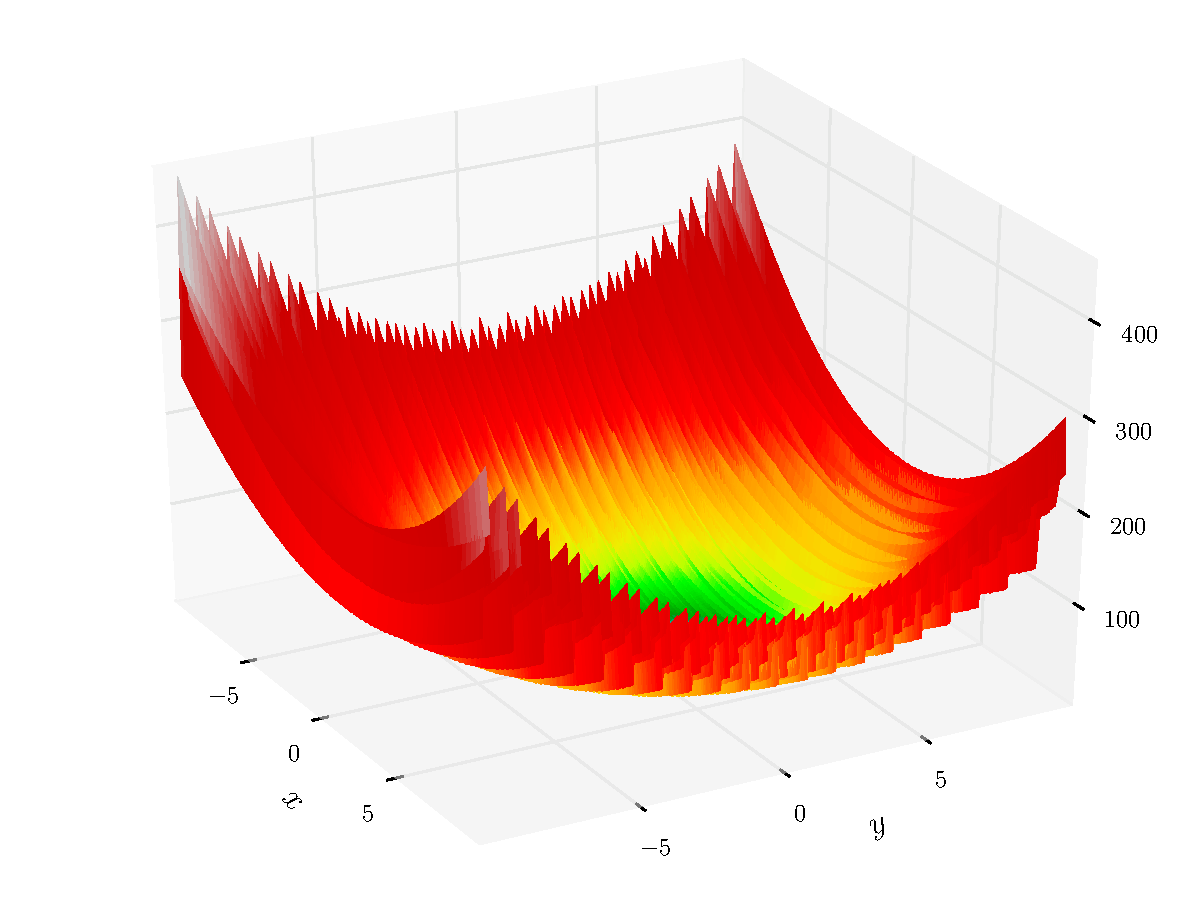
\includegraphics[width=0.6\textwidth]{levi.pdf}
    \caption{График функции Леви для двух переменных.}
    \label{levi_plot}
\end{figure}

\section{Функция Растригина}

Леонард Растригин предложил нелинейную мультимодальную функцию для тестирования эффективности алгоритмов оптимизации. Нахождение минимума этой функции затруднено большим количеством локальных минимумов в области поиска. Функция задается формулой~(\ref{rastrigin_eq}).

\begin{equation}
\label{rastrigin_eq}
f(x_1, .., x_n) = An + \sum\limits_{i = 1}^n\left[ x_i^2 - Acos\left(2 \pi x_i \right)\right]
\end{equation}

\subsection{Одномерный случай}

\begin{figure}
    \centering
    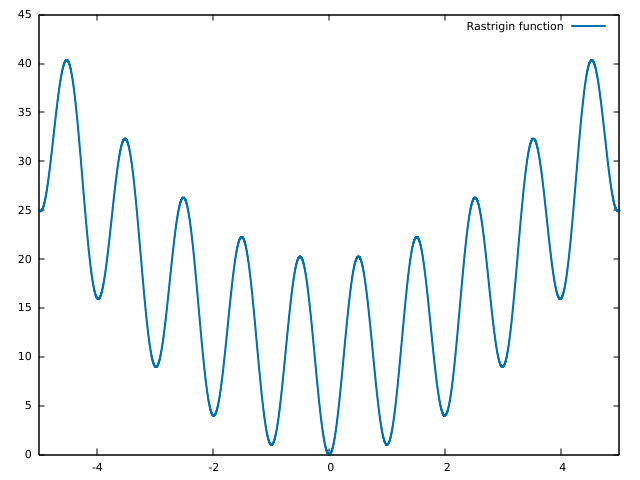
\includegraphics[width=0.6\textwidth]{rastrigin_1.png}
    \caption{График функции Растригина для одной переменной.}
    \label{rastrigin_plot}
\end{figure}

\subsection{Двумерный случай}

\begin{figure}
    \centering
    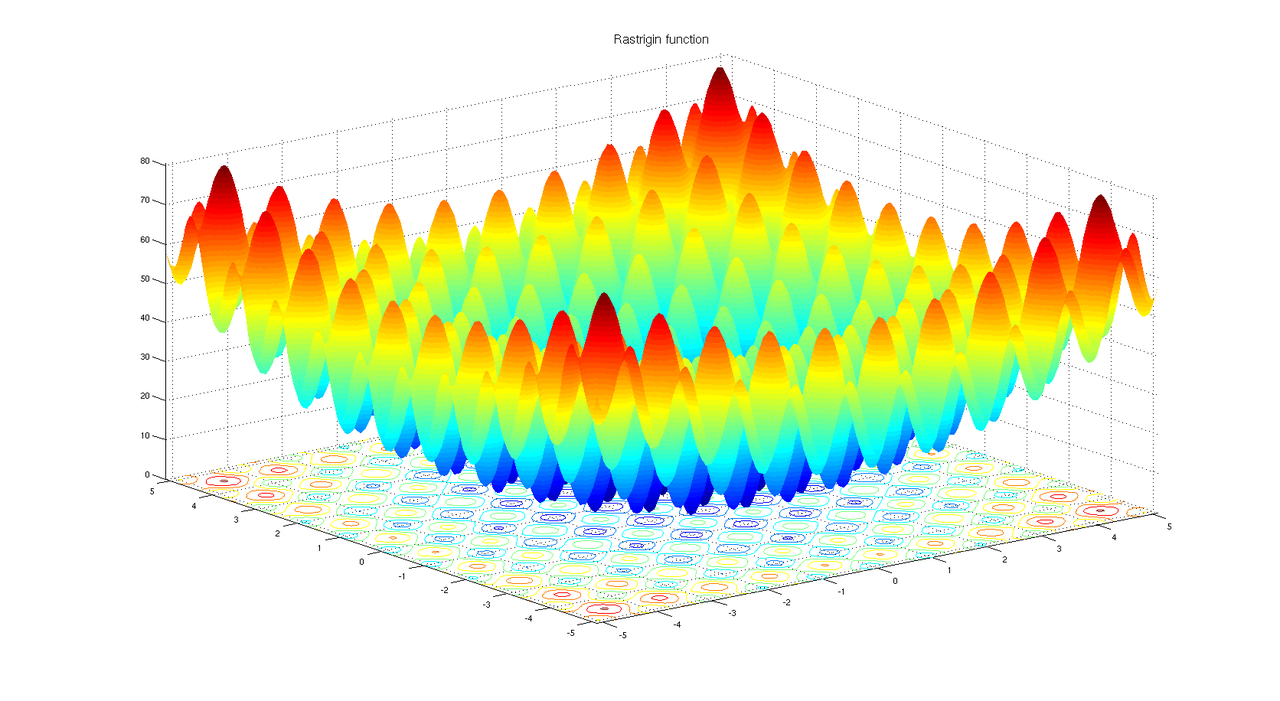
\includegraphics[width=0.6\textwidth]{rastrigin_2.png}
    \caption{График функции Растригина для двух переменных.}
    \label{rastrigin_plot}
\end{figure}

\section{Выводы}
